
\subsection{chapter over view}
\begin{itemize}
\item to assess the accuracy of current neural modelling work we explored:
\item variance in models
\item variance in experiments,  
\item variance in the combined set of models and experiments.
\item combine this discussion with model re-purposing discussion.
%\item model re-purposing?

\end{itemize}

%Druckmann \cite{druckmann2008evaluating}

%\cite{buil}


\subsubsection{Cortical Model and Cortical Experiment Agreement}

NeuroML-DB \cite{birgiolas2016rapid} catalogues over 1,500 published models obtained in NeuroML format from Open Source Brain [5]. Complementing OSB, NeuroML-DB provides systematic characterizations of model complexity, electrophysiology, and morphology, making it easy to find, evaluate, and reuse models and their components.\\
\\
It is known that generally that neural models and experimental measurements diverge in some respects,  however, we needed to locate specific sources of divergence. Specific knowledge of model/data disagreement informs the question: "In  cortical neuron models which aspects of a voltage recordings should be prioritized as optimization constraints?"

\subsubsection{Features} Consider a voltage recording at the location of the membrane of a neuron. Teams of researchers have already segmented voltage recordings into labelled sections, each section has a classification that is based on the shape of waveform in a limited region. Rather than specifying by name each measurement it is often useful to refer collectively to these measurable shapes as "features". In a multivariate analysis we analyze hundreds of such features, and we summarize important differences in a subset of this high dimensional feature space. 

Below, I describe some neuronal model features that agreed well with experiments, and some features that diverged.


\subsubsection{Publications Associated with Model Sources}

\begin{table}[ht]
\centering
\resizebox{\textwidth}{!}{
\begin{tabular}{lll}
\toprule
{} & Large Scale Model &   Publication 
Allen Institute V1 Model &  \cite{gouwens2018systematic}
Somatosensory Cortex & \cite{markram2015reconstruction}
\bottomrule
\end{tabular}}
\end{table}

\subsubsection{Feature Extraction Libraries}
\begin{table}[ht]
\centering
\resizebox{\textwidth}{!}{
\begin{tabular}{lll}
\toprule
{} & EFEL Ephys Feature Extraction Library & AllenSDK & Druckmann (2012) 
\bottomrule
\end{tabular}}
\end{table}


\subsubsection{Virtual Experiment Three Step Protocol Stimulate for 2s}

\begin{table}[ht]
\centering
\resizebox{\textwidth}{!}{
\begin{tabular}{lll}
\toprule
{} Injection 1 & Injection 2 & Injection 3 &
 at 1.0×Rheobase & at 1.5×Rheobase & at 3.0×Rheobase 
\bottomrule
\end{tabular}}
\end{table}



%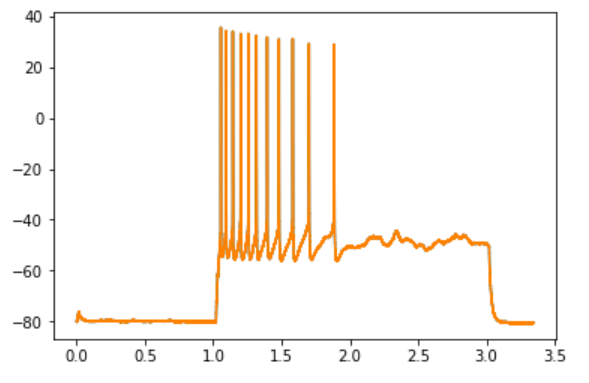
\includegraphics[]{chapters/app_tex/Allen_rush}
\begin{figure}
    \begin{center}
    
    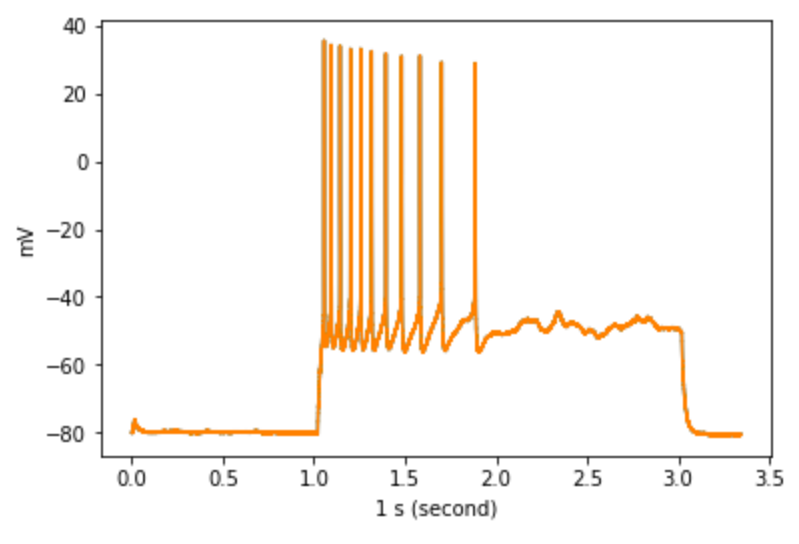
\includegraphics[width=0.6\linewidth]{figures/multi_spiking_large_allen}
    \caption{A voltage recording from a suprathreshold experiment waveform used as a basis for the Allen Brain Institute cell types data base. Publication Gouwens rat \cite{gouwens2018systematic}}

    \end{center}
    
\end{figure}    

\begin{figure}  
    \begin{center}
    
    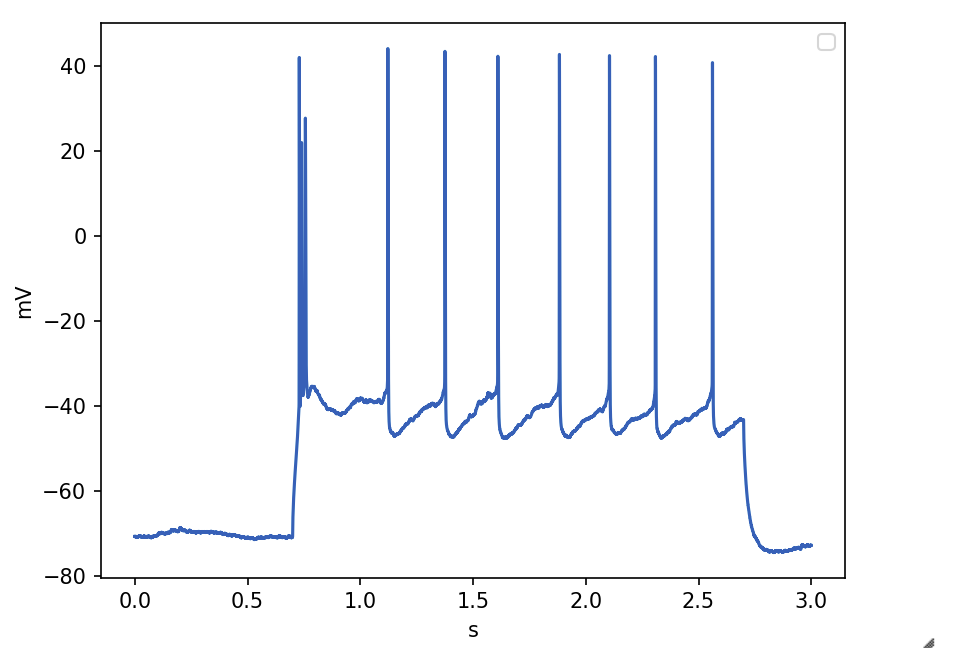
\includegraphics[width=0.6\linewidth]{figures/multi_spiking_large_bbp}
    \caption{An example of a multispiking waveform used as a basis for the Blue Brain Project. Publication Jouvanile rat \cite{toledo}}


    \end{center}
\end{figure}    



%\end{tcolorbox}
\begin{figure}    
\begin{center}

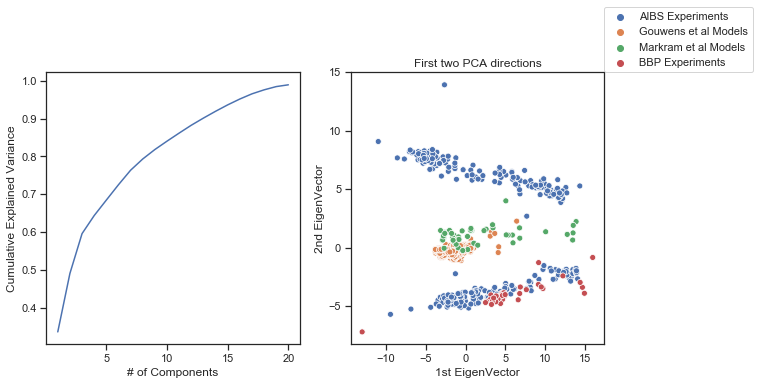
\includegraphics[width=1.0\linewidth]{figures/cortical_model_data_agreement_52_1.png}
\caption{}

\end{center}
\end{figure}    
\begin{figure}    
\begin{center}
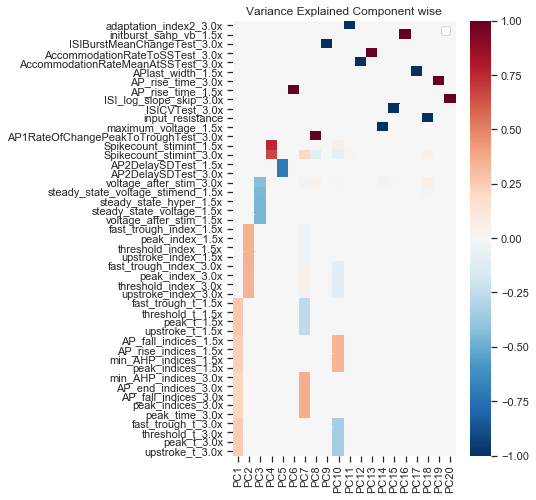
\includegraphics[width=1.0\linewidth]{figures/cortical_model_data_agreement_54_1.png}
\caption{}
\end{center}
\end{figure}    
\cite{wang2019sag}
\begin{itemize}
    \item upstroke\_t\_1.5x allen feature
    \item  peak\_t\_1.5x allen feature
    \item threshold\_t\_1.5x allen feature
    \item fast\_trough\_t\_1.5x allen feature
    \item fast\_trough\_t\_3.0x allen feature
    \item upstroke\_t\_3.0x allen feature
    \item peak\_t\_3.0x allen feature
    \item threshold\_t\_3.0x allen feature
    \item peak\_indices\_1.5x efel feature
    \item min\_AHP\_indices\_1.5x efel feature
\end{itemize}


\begin{itemize}

    \item fast\_trough\_index\_1.5x allen feature
    \item fast\_trough\_index\_3.0x allen feature
    \item threshold\_index\_1.5x allen feature
    \item peak\_index\_1.5x allen feature
    \item upstroke\_index\_1.5x allen feature
    \item peak\_index\_3.0x allen feature
    \item upstroke\_index\_3.0x allen feature
    \item threshold\_index\_3.0x allen feature
\end{itemize}


